\documentclass[11pt]{article}
\usepackage{latexsym}
\usepackage{amsmath}
\usepackage{amssymb}
\usepackage{amsthm}
\usepackage{epsfig}
\usepackage[tight]{subfigure}

\usepackage{amsmath}
\usepackage{hyperref}
\usepackage[table]{xcolor}

\DeclareMathOperator*{\minimize}{min}
\DeclareMathOperator*{\maximize}{max}
\DeclareMathOperator*{\argmax}{arg\,max}
\DeclareMathOperator*{\argmin}{arg\,min}

\usepackage{algorithm, algpseudocode}
 %on linux you may need to run sudo apt-get install texlive-full to install algorithm.sys

\usepackage{verbatim}

\newcommand{\handout}[5]{
  \noindent
  \begin{center}
  \framebox{
    \vbox{
      \hbox to 5.78in { {#1} \hfill #2 }
      \vspace{4mm}
      \hbox to 5.78in { {\Large \hfill #5  \hfill} }
      \vspace{2mm}
      \hbox to 5.78in { {\em #3 \hfill #4} }
    }
  }
  \end{center}
  \vspace*{4mm}
}

\newcommand{\lecture}[5]{\handout{#1}{#2}{#3}{#4}{#5}}
\newcommand{\collision}[0]{\mathrm{collision}}
\newcommand{\nocollision}[0]{\overline{\collision}}

\newcommand*{\QED}{\hfill\ensuremath{\square}}

\newtheorem{theorem}{Theorem}
\newtheorem{corollary}[theorem]{Corollary}
\newtheorem{lemma}[theorem]{Lemma}
\newtheorem{observation}[theorem]{Observation}
\newtheorem{proposition}[theorem]{Proposition}
\newtheorem{definition}[theorem]{Definition}
\newtheorem{claim}[theorem]{Claim}
\newtheorem{fact}[theorem]{Fact}
\newtheorem{assumption}[theorem]{Assumption}
\newtheorem{note}[theorem]{Note}

% 1-inch margins, from fullpage.sty by H.Partl, Version 2, Dec. 15, 1988.
\topmargin 0pt
\advance \topmargin by -\headheight
\advance \topmargin by -\headsep
\textheight 8.9in
\oddsidemargin 0pt
\evensidemargin \oddsidemargin
\marginparwidth 0.5in
\textwidth 6.5in

\parindent 0in
\parskip 1.5ex
%\renewcommand{\baselinestretch}{1.25}

\begin{document}

\lecture{Statistical Techniques in Robotics (16-831, S22)}{Lecture \#16
  (Monday, Mar 21)}{Lecturer: Kris Kitani}{Scribes: Siqi Chai, Jiajie Xu (Group B)}{Model-Free Value Prediction}

\section{Review}
In the previous lecture, we discussed value-based model-based control, also known as model-based reinforcement learning. It is named "value-based" because our agent is explicitly learning value function $V$ to choose the best policy. And it's called "model-based" because state transition dynamics $p(s^\prime|s,a)$ and reward function $r(s^\prime, a, s)$ are either known from the environment, or we are trying to estimate them. We covered two algorithms: policy iteration and value iteration. \\
\begin{figure}[H]
    \centering
    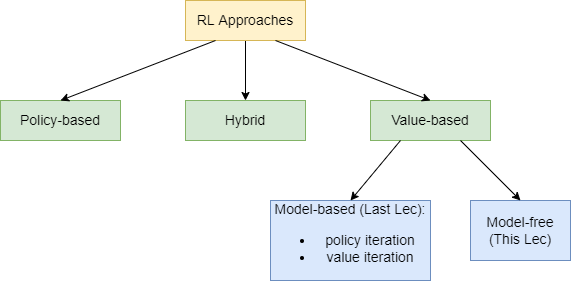
\includegraphics[width=0.7\textwidth]{pic/RL_approaches.png}
\end{figure}
The other two types of reinforcement learning approaches:
\begin{itemize}
    \item Policy-based: learn parameterized policy that select action without consulting value function \cite{bartoRL}
    \item Hybrid: combing value-based and policy-based methods. Current paradigm for research in this area
\end{itemize}

\begin{figure}[H]
    \centering
    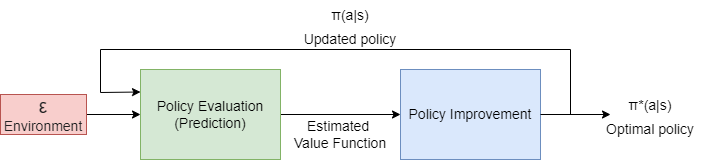
\includegraphics[width=0.9\textwidth]{pic/value_based_control.png}
    \label{fig:value_based_control}
\end{figure}

The key to policy evaluation step is Bellman equation:
\begin{equation}
V^{\pi}(s)=\sum_{a} \pi(a \mid s) \sum_{s^{\prime}} p\left(s^{\prime} \mid s, a\right)\left[r\left(s^{\prime}, a, s\right)+\gamma V^{\pi}\left(s^{\prime}\right)\right]
\end{equation}
\begin{equation}
\begin{split}
Q^{\pi}(s, a) &= \sum_{s^{\prime}} p\left(s^{\prime} \mid s, a\right) \left[r\left(s^{\prime}, a, s\right) + \gamma V^{\pi}\left(s^{\prime}\right) \right] \\
&= \sum_{s^{\prime}} p\left(s^{\prime} \mid s, a\right) \left[r\left(s^{\prime}, a, s\right) + \gamma \sum_{a^{\prime}} \pi\left(a^{\prime} \mid s^{\prime}\right) Q^{\pi}\left(s^{\prime}, a^{\prime}\right) \right]
\end{split}
\end{equation}
Value-based control does not require accurate model prediction to predict optimized policy.

\subsection{Policy Iteration}
In policy iteration, the agent evaluates $V$ given our current $\pi$, loop till $V$ for each state converges (policy evaluation), and then update policy for each state by choosing the one that maximize $V$ (Policy improvement), which causes $V$ to change again. Continue this loop until $\pi$ converges. $V^\prime$ in this algorithm refers to the old value function.

\begin{algorithm}[H]
\caption{POLICY\_ITERATION $\left(\pi, r(s), p\left(s^{\prime} \mid s, a\right), \gamma\right)$}
\label{algo:wma}
\begin{algorithmic}[1]
\State $\pi \leftarrow \operatorname{rand}(\mathcal{A})$
\State $V \leftarrow \operatorname{rand}(\mathbb{R})$
\State $V^{\prime} \leftarrow \operatorname{rand}(\mathbb{R})$
\While {$\pi^{\prime} \neq \pi$}
    \While {$\max _{s}\left|V(s)-V^{\prime}(s)\right| \geq \epsilon$}
        \Comment{Policy evaluation}
        \State $V^{\prime} \leftarrow V$
        \For{$s \in \mathcal{S}$}
            \State $Q(s, a)=r(s)+\gamma \sum_{s^{\prime}} p\left(s^{\prime} \mid s, a\right) V^{\prime}\left(s^{\prime}\right) \quad \forall a $
            \State $V(s)=\sum_{a} \pi(a \mid s) Q(s, a)$
        \EndFor
    \EndWhile \\
    
    \State $\pi^{\prime}(s)=\arg \max _{a} Q(s, a) \quad \forall s$
    \Comment{Policy improvement}
\EndWhile
\State return $\pi$
\end{algorithmic}
\end{algorithm}

\subsection{Value Iteration}
Value Iteration share the same block diagram as policy iteration. But the key difference between these two is that Value Iteration does not wait for $V$
to converge for the current $\pi$ before updating $\pi$, i.e. for each state, $\pi$ is updated right after $V(s)$ is calculated. Value iteration also takes direct advantage of dynamic programming. This makes value iteration converges faster compared with policy iteration.

% \subsection{Reinforcement Learning}
\clearpage
\section{Summary}
\subsection{Model-free Environment and Prediction}
In model-free environment, we do not have access to transition dynamics and reward function from the environment, and we make no attempt to estimate or use them. We will only interact with environment to collect interaction samples, which are in the form of quadruplets $\{s^\prime, r, s, a\}_{n=1}^N$
\begin{figure}[H]
    \centering
    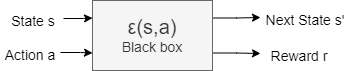
\includegraphics[width=0.5\textwidth]{pic/model_free_environment.png}
\end{figure}

When dealing with sampled interaction with the environment, there are two methods, with a debate between which one is better in performance.
\begin{itemize}
    \item Model-based RL: Estimate $p(s^\prime|s,a)$ and $r(s^\prime, a, s)$ functions to fit N datapoints $\{s^\prime, r, s, a\}_{n=1}^N$, learn the dynamics and convert to model-based prediction problem, same as last lecture
    \item Model-free prediction: use a new algorithm for the policy evaluation block in Figure \ref{fig:value_based_control} to directly measure/estimate the value function
\end{itemize}

Next, we will cover several model-free prediction algorithms. The difference between on-policy and off-policy is how you draw samples (using current vs other policy)
\begin{center}
\begin{tabular}{ |c|c|c| }
 \hline
 Algorithms & Monte Carlo & Temporal Differencing \\
 \hline\hline
 on-policy & Monte Carlo & N-step TD, TD-lambda \\  
 \hline
 off-policy & Importance Sampling Monte-Carlo & Importance Sampling
Temporal Differencing \\
 \hline
\end{tabular}
\end{center}

\subsection{Monte Carlo}
The Monte Carlo algorithm is the most basic reinforcement learning algorithm. The goal is to learn the value function from the samples. We assume that we do not have access to the transition dynamics \(p(s' | s, a)\) and the reward function \(r(s', s, a)\). We are given the policy \(\pi(a|s)\) and the problem is to find the value function:
\[Q(a, s)\]
The problem itself is like test driving the policy in a environment. The reward function is recovered through interaction with the environment. Recall the state value function we introduced before:
\begin{equation}
V^{\pi}(s) = E_{\pi, P} [\sum_{t=0}^T \gamma^t r_t | s_0=s]
\end{equation}
The value of a state is the expected return under the MDP (Policy, dynamics, initial state distribution). We can rewrite it with a short-hand notation G representing the cumulative discounted reward over one episode, 
\begin{equation}
V^{\pi}(s) = E_{\pi, P} [G | s_0=s]
\end{equation}
Note that, we do not have access to the transition dynamics, \(P\). Thus, in a model free setup, we cannot directly compute the value function through this formulation. To solve this problem in this setting, we use Monte Carlo estimate, that is, to interact with the environment many times and use the average return as the reward function.
\begin{figure}[h]
\centering
\begin{tabular}{| c | c | c | c |}
\hline
-1 & +2 & -1 & +10, Win \\
\hline
-1, s0 & -8 & +2 & -8 \\
\hline
-1 & -1 & -1 & -10, Die \\
\hline
\end{tabular}
\end{figure}
Suppose we have a grid game defined as above. We start from \(s_0\), which is the first grid on the second row. In this case, if we want to estimate the value of state \(s_0\), we can use Monte Carlo estimate. We play the game for \(N\) times, and record the cumulative reward of each trajectory. After \(N\) games, we take the average over all the cumulative reward for each round, and use that value as the estimated rewad of \(s_0\):
\begin{equation}
V(s_0) = \dfrac{1}{N} \sum_{i=1}^N G(s_0)
\end{equation}

\subsubsection{First Visit MC Prediction}
The above procedure we seen is called the \hyperref[alg:fvmp]{First Visit MC Prediction algorithm}. On line 5 of the algorithm, in each episode, we drawn a trajectory following the distribution specified by environment \(\varepsilon\) and policy \(\pi\).Given a trajectory in each episode, we iteratively compute the award of each state along the trajectory. Note on line 7, we prevent updating a pre-calculated state award by enforcing the update to only happen on first visit to a state. If it is a first visit to a state (line 8, 9), we calculate the cumulative reward of this state by summing up all the upcoming reward along the trajectory after this state. We also add the counter \(N\) for this state by 1. Eventually, we return the average rewards as the Monte Carlo estimate of the reward function for policy \(\pi\)
\begin{algorithm}
\caption{FirstVisit-MC-Prediction}
\label{alg:fvmp}
\begin{algorithmic}[1]
\State $\pi$: a policy
\State $\varepsilon$: The environment
    \Procedure{FirstVisit-MC-Prediction}{$\pi$, $\varepsilon$}
    \For{$e=1,\;\cdots,\;E$}
    \State $\{s^{(t)}, a^{(t)}, r^{(t)}\} \sim \varepsilon | \pi$
        \For{$t=0,\;\cdots,\;T$}
        \If{First Visit to $s^{(t)}$ in episode $e$}
            \State $G(s^{(t)}) \gets G(s^{(t)}) + \sum_{i=t}^T r^{(i)}$
            \State $N(s^{(t)}) \gets N(s^{(t)}) + 1$
        \EndIf
        \EndFor
    \EndFor
    \State \textbf{return} $V(s) \gets G(s) / N(s) \quad \forall s$
    \EndProcedure
\end{algorithmic}
\end{algorithm}

\subsubsection{First Visit Incremental MC Prediction}
A variant of the above algorithm is the \hyperref[alg:fvimp]{First Visit Incremental MC Prediction}. The only difference to the previous algorithm is that here we incrementally update the value function, instead of averaging it by the very end. This is also called the 'offline' update. Note that on line 10, the update here is actually taking the weighted average. That is:
\begin{align}
\begin{split}
    V(s) &= \frac{N(s) - 1}{N(s)} V(s) + \frac{1}{N(s)} G_e(s) \\
    &= V(s) - \frac{1}{N(s)} V(s) + \frac{1}{N(s)} G_e(s) \\
    &= V(s) + \frac{1}{N(s)} (G_e(s) - V(s))
\end{split}
\end{align}
The reason we do this weighted average update is because it can generalize to a changing environment. If the environment changes during the algorithm roll out, we may want to forget older episode and adapt to newer ones. We can do so by weighting new updates with a \(\alpha\) factor, that is:
\begin{equation}
V(s) = V(s) + \alpha (G_e(s) - V(s))
\end{equation}
\begin{algorithm}
\caption{FirstVisit-Incremental-MC-Prediction}
\label{alg:fvimp}
\begin{algorithmic}[1]
\State $\pi$: a policy
\State $\varepsilon$: The environment
    \Procedure{FirstVisit-Incremental-MC-Prediction}{$\pi$, $\varepsilon$}
    \For{$e=1,\;\cdots,\;E$}
    \State $\{s^{(t)}, a^{(t)}, r^{(t)}\} \sim \varepsilon | \pi$
        \For{$t=0,\;\cdots,\;T$}
        \If{First Visit to $s^{(t)}$ in episode $e$}
            \State $G(s^{(t)}) \gets G(s^{(t)}) + \sum_{i=t}^T r^{(i)}$
            \State $N(s^{(t)}) \gets N(s^{(t)}) + 1$
            \State $V(s) \gets V(s) + \frac{1}{N(s^{(t)})} (G_e(s^{(t)}) - V(s^{(t)}))$
        \EndIf
        \EndFor
    \EndFor
    \State \textbf{return} $V(s)$
    \EndProcedure
\end{algorithmic}
\end{algorithm}

\subsubsection{Every Visit MC Prediction}
Based on the previous algorithm, if we further remove the constraint that only update the reward on first visit, we have \hyperref[alg:evmp]{Every Visit MC Prediction}. This is the general form of Monte Carlo estimation. However, looking at line 7, we can see that this update is causing the algorithm slow. This step makes the time complexity of each episode of \(O(T^2)\). We can avoid this by caching the rewards. If we change line 6 to compute backward, that is \(t=T,\;\cdots,\;0\), we can speed things up. \par
Can we use this algorithm for a infinite horizon problem? The answer is no due to the fact on line 8. We need episodic returns to complete the estimate. \par
Can we replace the pre-sampling of trajectories on line 4 with a online updated calculation? The answer is yes. We can use the TD-algorithm introduced later.
\begin{algorithm}
\caption{EveryVisit-MC-Prediction}
\label{alg:evmp}
\begin{algorithmic}[1]
\State $\pi$: a policy
\State $\varepsilon$: The environment
    \Procedure{EveryVisit-MC-Prediction}{$\pi$, $\varepsilon$}
    \For{$e=1,\;\cdots,\;E$}
    \State $\{s^{(t)}, a^{(t)}, r^{(t)}\} \sim \varepsilon | \pi$
        \For{$t=0,\;\cdots,\;T$}
        \State $G^{(t)} \gets \sum_{i=t}^T r^{(i)}$
        \State $V(s^{(t)}) \gets V(s^{(t)}) + \alpha (G^{(t)} - V(s^{(t)}))$
        \EndFor
    \EndFor
    \State \textbf{return} $V(s)$
    \EndProcedure
\end{algorithmic}
\end{algorithm}

\subsubsection{Properties of Monte Carlo prediction}
\begin{itemize}
    \item Model free approach: we do not need the value function, we estimate it.
    \item Monte Carlo is known for high variance for long trajectory estimation. This happens because at each state along a trajectory, there will be some randomness. Long trajectory can accumulate these randomness, causing high variances. 
    \item works only for finite horizon problem.
    \item Uses full return to estimate the value function, as opposed to bootstrapping.
    \item Yields unbiased estimate, due to above property (zero bias in mean)
    \item Converges to the MSE solution
\end{itemize}

\subsection{N-step TD}
\subsubsection{Temporal Difference Prediction}
In Temporal Difference Prediction algorithm, we introduce the idea of bootstrapping (from dynamic programming) to incrementally estimate values after every action, based on another estimate.

Recall the value function update equation from Monte Carlo:
\begin{equation}
V(s)^{(t)} \leftarrow V(s^{(t)}) + \alpha (G^{(t)} - V(s^{(t)}))
\end{equation}
The empirical reward $G^{(t)}$ can be estimated as the sum of immediate reward $r^{(t)}$ and discounted estimated value for the next time step $V(s^{(t+1)})$:
\begin{equation} \label{1s_td_target}
G^{(t)} = r^{(t)} + \gamma V(s^{(t+1)})
\end{equation}
This sum is called \textbf{1-step TD target}, and $r^{(t)} + \gamma V(s^{(t+1)}) - V(s^{(t)})$ is called \textbf{TD error}. The 1-step TD update function can be written as:
\begin{equation} \label{1s_td_update}
V(s^{(t)}) \leftarrow V(s^{(t)}) + \alpha (r^{(t)} + \gamma V(s^{(t+1)}) - V(s^{(t)}))
\end{equation}
If we incrementally substitute value function with the sum of immediate reward and estimated value, we get the total reward for N-step TD:
\begin{equation}
G^{(t)}(N) = r^{(t)} + \gamma r^{(t+1)} + \cdots + \gamma ^{(N-1)} r^{(N-1)} +\gamma ^ N V(s^{(t + N)})
\end{equation}
Notice that if we have $N=T-t$, meaning that we sum all reward functions till time step T and don't do any estimation, the total reward function $G^{(t)}(\infty)$ becomes the same as Monte Carlo algorithm.

Let's go back to the grid game and use it as an 1-step TD example. But this time at each state, we have a "memo" to tell us the estimated value function of the state \textcolor{blue}{(marked blue)}. This estimate needs to be initialized before time step 0, and will be updated for each action. In the example, $\gamma=1$, $\alpha=0.9$
\begin{figure}[h]
\centering
\begin{tabular}{| c | c | c | c |}
\hline
-1 \textcolor{blue}{(10)} & +2 \textcolor{blue}{(11)} & -1 \textcolor{blue}{(9)} & +10, Win \textcolor{blue}{(10)} \\
\hline
-1 \textcolor{blue}{(8)} \textcolor{red}{(8.9)}, s0 & -8 & +2 \textcolor{blue}{(9)} & -8 \\
\hline
-1 \textcolor{blue}{(7)} & -1 \textcolor{blue}{(8)} & -1 \textcolor{blue}{(9)} & -10, Die \\
\hline
\end{tabular}
\end{figure}

At s0, suppose the policy decide to go up, then using one step TD estimate in equation \ref{1s_td_target}:
\[ G(1) = r + \gamma \cdot V(s^\prime) = -1 + 1 \cdot 10 = 9 \]
Update value estimate at state 0 using equation \ref{1s_td_update} \textcolor{red}{(marked red)}:
\[ V(s0) \leftarrow V(s0) + \alpha (G(1) - V(s0)) \]
\[ V(s0) = 8 + 0.9 \cdot (9-8) = 8.9 \]

The pseudocode for the algorithm above:
\begin{algorithm}[H]
\caption{1-STEP-TD-Prediction $(\pi,\alpha,\gamma)$}
\label{algo:1std}
\begin{algorithmic}[1]
\For {$e=1, \ldots, E$}
    \State $\left\{s^{(t)}, a^{(t)}, r^{(t)}\right\}_{t=0}^{T} \sim \mathcal{E} \mid \pi$
    \For {$t=0, \ldots, T - 1$}
        \State $G^{(t)}\left(1\right) \leftarrow r^{(t)} + \gamma V(s^{(t+1)})$
        \State $V(s^{(t)}) \leftarrow V(s^{(t)}) + \alpha \left[ G^{(t)}(1) - V(s^{(t)}) \right]$
    \EndFor
\EndFor
\State $\text{return } V(s) $
\end{algorithmic}
\end{algorithm}
In the algorithm:
\begin{itemize}
    \item E is the total episode number, we want it to be a sufficiently large number, but there is no hard convergence condition
    \item For the sampling process in line 2, we don't need to sample the whole trajectory at each time step t, due to the estimation of $V(s^{(t+1)})$
\end{itemize}

Substitute line 4 of the above algorithm from TD 1-step to TD N-step, we get N-step TD prediction algorithm:
\begin{algorithm}[H]
\caption{N-STEP-TD-Prediction $(\pi,\alpha,\gamma,N)$}
\label{algo:1std}
\begin{algorithmic}[1]
\For {$e=1, \ldots, E$}
    \State $\left\{s^{(t)}, a^{(t)}, r^{(t)}\right\}_{t=0}^{T} \sim \mathcal{E} \mid \pi$
    \For {$t=0, \ldots, T - 1$}
        \State $G^{(t)}\left(N\right) \leftarrow \sum_{i=t}^{t+N-1} \gamma^{i-t} r^{(i)} + \gamma^N V(s^{(t+N)})$
        \State $V(s^{(t)}) \leftarrow V(s^{(t)}) + \alpha \left[ G^{(t)}(1) - V(s^{(t)}) \right]$
    \EndFor
\EndFor
\State $\text{return } V(s) $
\end{algorithmic}
\end{algorithm}

\subsubsection{Properties of N-step TD Prediction}
\begin{enumerate}
    \item TD prediction is model-free
    \item Uses bootstrapping to estimate value function
    \item Compared with Monte Carlo:
    \begin{itemize}
        \item Do not need reward for the full episode at time step t, only the next N steps
        \item For the above reason, Monte Carlo is called an offline/batch algorithm, while N-step TD is called online/incremental algorithm
        \item For the same reason, N-step TD can be used for non-terminating problem (infinite horizon)
        \item N-step TD is more efficient, but the estimation is biased because it depends on value function estimation in future step
        \item TD prediction has low variance due to short sequence length
    \end{itemize}
    \item Need to select the optimal N depending on the problem (hyperparameter), which contains a trade-off between higher variance and bias 
\end{enumerate}

%\section*{References}
%Include your references here. Please cite any resources you found useful.	
%Populate the refs.bib file or list your references manually. Be consistent in formatting!
{
\bibliography{refs}
\bibliographystyle{abbrv}
}

\end{document} % Done!
